% \documentclass[UTF8]{ctexbeamer}
\documentclass[12pt]{beamer}
% \usepackage[UTF8]{ctex}
\usepackage{latexsym}
\usepackage{amsmath}
\usepackage{amssymb}
\usepackage{graphicx}
\usepackage{algorithm}
\usepackage{amsthm}
\usepackage{booktabs}
\usepackage{fontspec}
\usepackage{physics}
\usepackage{lipsum}
\usepackage{tikz}
\usepackage{forest}
\usepackage{subcaption}
\usepackage{hyperref}
\usepackage{caption}

\makeatletter

\let\@@magyar@captionfix

\relax\makeatother



\usefonttheme[onlymath]{serif}    %设置数学公式应该使用衬线字体
% Use metropolis theme
\usetheme[
    block=fill,
    background=light,
    subsectionpage=progressbar,
    progressbar=frametitle,
    titleformat=smallcaps,
    titleformat frame=regular,
]{metropolis}

% Swap \phi and \varphi
\let\temp\phi
\let\phi\varphi
\let\varphi\temp

\newcommand*{\vcenteredhbox}[1]{\begingroup
\setbox0=\hbox{#1}\parbox{\wd0}{\box0}\endgroup}
\newcommand{\iu}{\mathrm{i}}
\newcommand{\vac}{\ket{\mathrm{vac}}}
\newcommand{\cdeg}{{}^\circ\mathrm{C}}
\newcommand\blfootnote[1]{%
    \begingroup
    \renewcommand\thefootnote{}\footnote{\tiny#1}%
    \addtocounter{footnote}{-1}%
    \endgroup
}
\newcommand{\pf}{\phantom{\em}}

\tikzstyle{state}=[circle, draw, fill=blue!20, thick, minimum width=2.5em]
\tikzstyle{basis}=[circle, draw, fill=green!30, thick, minimum width=2.5em]
\tikzstyle{operator}=[rectangle, draw, fill=red!40, thick, minimum width=2.5em, minimum height=2.5em]
\tikzstyle{other}=[rectangle, draw, fill=yellow!50, thick, minimum width=2.5em, minimum height=2.5em]

\begin{document}

    \title{Multi-Configuration Time Dependent Hartree Theory}
    \subtitle{A Tensor Network Perspective}
    \author{Xinxian Chen}
    \institute{Department of Chemistry, Tsinghua University}
    \date{\today}

    \frame{\titlepage}

    \begin{frame}{Non-Relativistic Multi-Dimentional Problem}
        \begin{itemize}
            \item TDSE:
            \begin{equation*}
                \iu \hbar \pdv{t} \ket{\Psi(\vec{q}, t)} = H \ket{\Psi(\vec{q}, t)}
            \end{equation*}
            \item TISE:
            \begin{equation*}
                H \ket{\Psi(\vec{q}, t)} = E \ket{\Psi(\vec{q}, t)}
            \end{equation*}
        \end{itemize}
        
        where $$H = T + V$$
        and $\vec{q} = \left(q_1, q_2, \ldots, q_d\right)$.
    \end{frame}

    \begin{frame}{$d$-D Problem: $\vec{q} = (q_1, \ldots, q_d)$}
        Standard procedure:
        \begin{enumerate}
            \item Choose a set of $d$-D basis $\left\{ \ket{\Phi_I(\vec{q})} \right\}^N_{I=1}$, where $\ket{\Phi_I(\vec{q})} = \prod_{\kappa=1}^d \ket{\phi^{(\kappa)}_{i_\kappa}(q_\kappa)}$
            \item Integrate $H_{IJ} = T_{IJ} + V_{IJ}$
            \item Solve TDSE/TISE in matrix form
            \begin{itemize}
                \item TDSE: $\iu \hbar \dot{\vb{c}} = \vb{H} \vb{c} $
                \item TISE: $\vb{H} \vb{c} = E \vb{c} $
            \end{itemize}
        \end{enumerate}
    \end{frame}

    \begin{frame}{Language: Tensor Network Notation}
        \begin{itemize}
            \item Tensors
            \begin{center}
                \footnotesize
                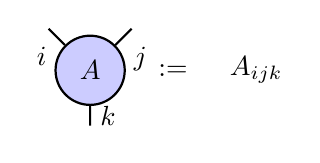
\begin{tikzpicture}[x=2em, y=2em]
                    \node[state] (a) at (0, 0) {$A$};
                    \node (f) at (3, 0) {$A_{ijk}$};
                    \draw[auto, thick]
                        (a) to node {$i$} (-0.75, 0.75)
                        (a) to node[swap] {$j$} (0.75, 0.75)
                        (a) to node {$k$} (0, -1)
                    ;
                    \path (a) to node[midway] {$:=$} (f);
                \end{tikzpicture}
                \hspace{0.2\textwidth}
                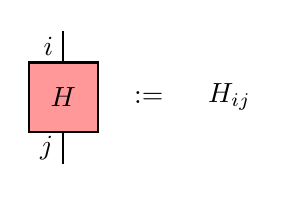
\begin{tikzpicture}[x=2em, y=2em]
                    \node[operator] (a) at (0, 0) {$H$};
                    \node (f) at (3, 0) {$H_{ij}$};
                    \draw[auto, thick]
                        (a) to node {$i$} (0, 1.2)
                        (a) to node[swap] {$j$} (0, -1.2)
                    ;
                    \path (a) to node[midway] {$:=$} (f);
                \end{tikzpicture}
            \end{center}

            \item Contraction
            \begin{figure}
                \centering
                \footnotesize
                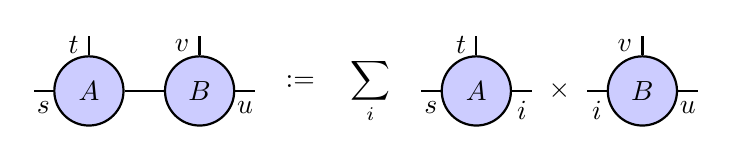
\begin{tikzpicture}[x=2em, y=2em]
                    \node[state] (a) at (0, 0) {$A$};
                    \node[state] (b) at (2, 0) {$B$};
                    \node[state] (a1) at (7, 0) {$A$};
                    \node[state] (b1) at (10, 0) {$B$};
                    \path (b) to node {$:= \quad \displaystyle\sum_i$} (a1);
                    \path (a1) to node {$\times$} (b1);
                    \draw[auto, thick]
                        (a) to node {$s$} (-1, 0)
                        (a) to node {$t$} (0, 1)
                        (b) to node[swap] {$u$} (3, 0)
                        (b) to node {$v$} (2, 1)
                        (a) to node {} (b)
                        (a1) to node {$s$} (6, 0)
                        (a1) to node {$t$} (7, 1)
                        (a1) to node[swap] {$i$} (8, 0)
                        (b1) to node {$i$} (9, 0)
                        (b1) to node[swap] {$u$} (11, 0)
                        (b1) to node {$v$} (10, 1)
                    ;
                \end{tikzpicture}
            \end{figure}
        \end{itemize}
        \blfootnote{
        Bridgeman, J. C. \& Chubb, C. T. J. Phys. A: Math. Theor. 50 223001 (2017). (arXiv:1603.03039)}
    \end{frame}

    \begin{frame}{Express the Standard Procedure in TNN}
        \begin{itemize}
            \item Wavefunction
            \begin{center}
                \footnotesize
                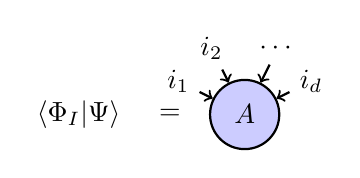
\begin{tikzpicture}[x=2em, y=2em, thick]
                    \node (f) at (-3, 0) {$\braket{\Phi_I}{\Psi}$};
                    \node[state] (a) at (0, 0) {$A$};
                    \node (1) at (-1.2, 0.6) {$i_1$};
                    \node (2) at (-0.6, 1.2) {$i_2$};
                    \node (3) at (0.6, 1.2) {$\cdots$};
                    \node (4) at (1.2, 0.6) {$i_d$};
                    \draw[<-]  (a)--(1);
                    \draw[<-]  (a)--(2);
                    \draw[<-]  (a)--(3);
                    \draw[<-]  (a)--(4);
                    \path (f) to node[midway] {$=$} (a);
                \end{tikzpicture}
            \end{center}
            where $i_\kappa \in \{ 1, \ldots, n_\kappa \}, \kappa = 1, \ldots, d$.

            Space for saving a wavefunction: $\prod_{\kappa=1}^d n_\kappa$ floats.
        \end{itemize}
    \end{frame}

    \begin{frame}{Express the Standard Procedure in TNN (Cont'd)}
        \begin{itemize}
            \item Normalization condition
            \begin{center}
                \footnotesize
                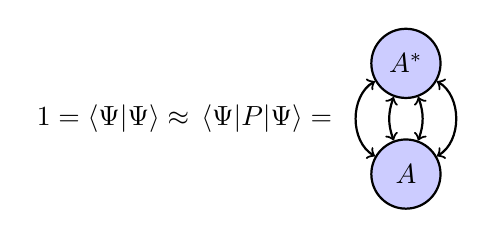
\begin{tikzpicture}[x=2em, y=2em, thick]
                    \node (f) at (-4, 1) {
                        $1 = \braket{\Psi} \approx \ev{P}{\Psi} = $
                    };
                    \node[state] (a) at (0, 0) {$A$};
                    \node[state] (a1) at (0, 2) {$A^*$};
                    \draw[<->]  (a) to [out=150, in=210] (a1);
                    \draw[<->]  (a) to [out=110, in=250] (a1);
                    \draw[<->]  (a) to [out=70,  in=290] (a1);
                    \draw[<->]  (a) to [out=30,  in=330] (a1);
                \end{tikzpicture}
            \end{center}

            \item TDSE
            \begin{center}
                \footnotesize
                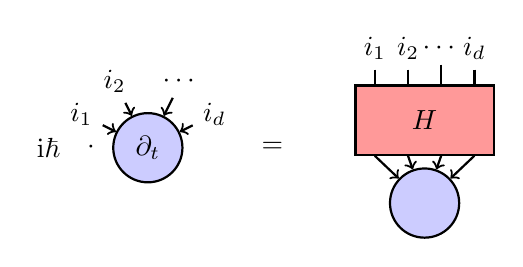
\begin{tikzpicture}[x=2em, y=2em, thick]
                    \node (c) at (-1.8, 0) {$\iu \hbar$};
                    \node[state] (a) at (0, 0) {$\partial_t$};
                    \node (1) at (-1.2, 0.6) {$i_1$};
                    \node (2) at (-0.6, 1.2) {$i_2$};
                    \node (3) at (0.6, 1.2) {$\cdots$};
                    \node (4) at (1.2, 0.6) {$i_d$};
                    \node[state] (b) at (5, -1) {\pf};
                    \node[operator, minimum width=5em] (h) at (5, 0.5) {$H$};
                    \node (p1) at (4.1, 1.8) {$i_1$};
                    \node (p2) at (4.7, 1.8) {$i_2$};
                    \node (p3) at (5.3, 1.8) {$\cdots$};
                    \node (p4) at (5.9, 1.8) {$i_d$};
                    \draw[<-]  (a)--(1);
                    \draw[<-]  (a)--(2);
                    \draw[<-]  (a)--(3);
                    \draw[<-]  (a)--(4);
                    \draw[<-]  (b) -- (p1 |- h.south);
                    \draw[<-]  (b) -- (p2 |- h.south);
                    \draw[<-]  (b) -- (p3 |- h.south);
                    \draw[<-]  (b) -- (p4 |- h.south);
                    \draw
                        (p1)--(p1 |- h.north) (p2)--(p2 |- h.north)
                        (p3)--(p3 |- h.north) (p4)--(p4 |- h.north)
                    ;
                    \path
                        (c) to node[midway] {$\cdot$} (a)
                        (-0.5, 0) to node[midway] {$=$} (5, 0)
                    ;
                \end{tikzpicture}
            \end{center}
        \end{itemize}
    \end{frame}

    \begin{frame}{Express the Standard Procedure in TNN (Cont'd)}
        \begin{itemize}
            \item TISE
            \begin{center}
                \footnotesize
                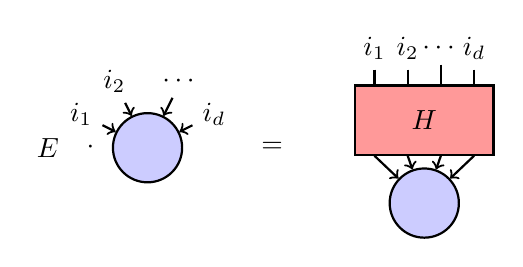
\begin{tikzpicture}[x=2em, y=2em, thick]
                    \node (c) at (-1.8, 0) {$E$};
                    \node[state] (a) at (0, 0) {\pf};
                    \node (1) at (-1.2, 0.6) {$i_1$};
                    \node (2) at (-0.6, 1.2) {$i_2$};
                    \node (3) at (0.6, 1.2) {$\cdots$};
                    \node (4) at (1.2, 0.6) {$i_d$};
                    \node[state] (b) at (5, -1) {\pf};
                    \node[operator, minimum width=5em] (h) at (5, 0.5) {$H$};
                    \node (p1) at (4.1, 1.8) {$i_1$};
                    \node (p2) at (4.7, 1.8) {$i_2$};
                    \node (p3) at (5.3, 1.8) {$\cdots$};
                    \node (p4) at (5.9, 1.8) {$i_d$};
                    \draw[<-]  (a)--(1);
                    \draw[<-]  (a)--(2);
                    \draw[<-]  (a)--(3);
                    \draw[<-]  (a)--(4);
                    \draw[<-]  (b) -- (p1 |- h.south);
                    \draw[<-]  (b) -- (p2 |- h.south);
                    \draw[<-]  (b) -- (p3 |- h.south);
                    \draw[<-]  (b) -- (p4 |- h.south);
                    \draw
                        (p1)--(p1 |- h.north) (p2)--(p2 |- h.north)
                        (p3)--(p3 |- h.north) (p4)--(p4 |- h.north)
                    ;
                    \path
                        (c) to node[midway] {$\cdot$} (a)
                        (-0.5, 0) to node[midway] {$=$} (5, 0)
                    ;
                \end{tikzpicture}
            \end{center}
        \end{itemize}
        where $i_\kappa \in \{ 1, \ldots, n_\kappa \}, \kappa = 1, \ldots, d$.

        Problem: $N = \prod_{\kappa=1}^d n_\kappa$ exponentially increase as $d$ grows.
    \end{frame}


    \begin{frame}{Structure of MCTDH Wavefunction}
        \begin{center}
            \tiny
            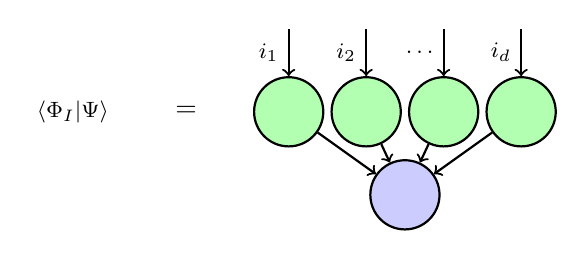
\begin{tikzpicture}[x=2em, y=2em, thick]
                \node (f) at (-6, 1.5) {\footnotesize$\braket{\Phi_I}{\Psi}$};
                \node[state] (a) at (0, 0) {\pf};
                \node[basis] (1) at (-2.1, 1.5) {\pf};
                \node[basis] (2) at (-0.7, 1.5) {\pf};
                \node[basis] (3) at ( 0.7, 1.5) {\pf};
                \node[basis] (4) at ( 2.1, 1.5) {\pf};
                \draw[<-]  (a)--(1);
                \draw[<-]  (a)--(2);
                \draw[<-]  (a)--(3);
                \draw[<-]  (a)--(4);
                \draw[auto, <-]  (1) to node {\footnotesize$i_1$} (-2.1, 3);
                \draw[auto, <-]  (2) to node {\footnotesize$i_2$} (-0.7, 3);
                \draw[auto, <-]  (3) to node {\footnotesize$\ldots$} ( 0.7, 3);
                \draw[auto, <-]  (4) to node {\footnotesize$i_d$} ( 2.1, 3);
                \path (f) to node[midway] {$=$} (1);
            \end{tikzpicture}
        \end{center}
        where
        \begin{center}
            \tiny
            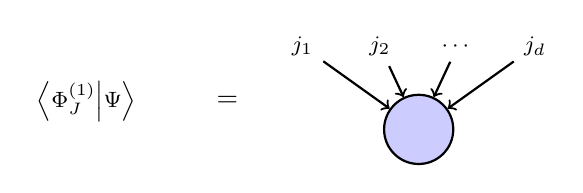
\begin{tikzpicture}[x=2em, y=2em, thick]
                \node (f) at (-6, 0.5) {\footnotesize$\braket{\Phi^{(1)}_J}{\Psi}$};
                \node[state] (a) at (0, 0) {\pf};
                \node (1) at (-2.1, 1.5) {\footnotesize$j_1$};
                \node (2) at (-0.7, 1.5) {\footnotesize$j_2$};
                \node (3) at ( 0.7, 1.5) {\footnotesize$\cdots$};
                \node (4) at ( 2.1, 1.5) {\footnotesize$j_d$};
                \draw[<-]  (a)--(1);
                \draw[<-]  (a)--(2);
                \draw[<-]  (a)--(3);
                \draw[<-]  (a)--(4);
                \path (f) to node[midway] {$=$} (-2, 0.5);
            \end{tikzpicture}
        \end{center}
        Idea: $j_\kappa \in \{1, \ldots, n^{(1)}_\kappa \}, \kappa = 1, \ldots, d$, and $n^{(1)}_\kappa < n_\kappa$.

        Space for saving a wavefunction: $\prod_{\kappa=1}^d n^{(1)}_\kappa + \sum_{\kappa=1}^d n^{(1)}_\kappa n_\kappa$ floats.
    \end{frame}

    \begin{frame}{Multi-Layer}
        More nodes, but smaller ranks.

        Example 1:
        \begin{center}
            \tiny
            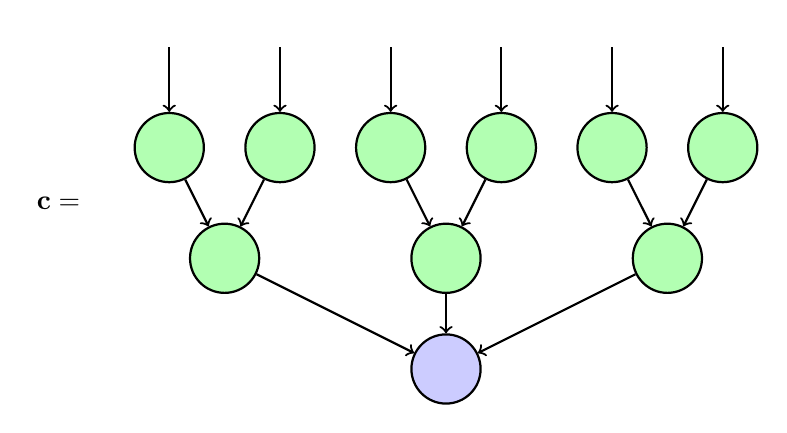
\begin{tikzpicture}[x=2em, y=2em, thick]
                \node (f) at (-7, 2.5) {\normalsize$\vb{c} = $};
                \node[state] (a) at (0, -0.5) {\pf};
                \node[basis] (11) at (-4, 1.5) {\pf};
                \node[basis] (12) at ( 0, 1.5) {\pf};
                \node[basis] (13) at ( 4, 1.5) {\pf};
                \node[basis] (21) at (-5, 3.5) {};
                \node[basis] (22) at (-3, 3.5) {};
                \node[basis] (23) at (-1, 3.5) {};
                \node[basis] (24) at ( 1, 3.5) {};
                \node[basis] (25) at ( 3, 3.5) {};
                \node[basis] (26) at ( 5, 3.5) {};
                \node (31) at (-5, 5.5) {};
                \node (32) at (-3, 5.5) {};
                \node (33) at (-1, 5.5) {};
                \node (34) at ( 1, 5.5) {};
                \node (35) at ( 3, 5.5) {};
                \node (36) at ( 5, 5.5) {};
                \draw[<-]  (a)--(11);
                \draw[<-]  (a)--(12);
                \draw[<-]  (a)--(13);
                \draw[<-]  (11) to (21);
                \draw[<-]  (11) to (22);
                \draw[<-]  (12) to (23);
                \draw[<-]  (12) to (24);
                \draw[<-]  (13) to (25);
                \draw[<-]  (13) to (26);
                \draw[<-]  (21) to (31);
                \draw[<-]  (22) to (32);
                \draw[<-]  (23) to (33);
                \draw[<-]  (24) to (34);
                \draw[<-]  (25) to (35);
                \draw[<-]  (26) to (36);
            \end{tikzpicture}
        \end{center}

        \blfootnote{Wang, H \& Thoss, M. J. Chem. Phys. 119, 1289 (2003)}
    \end{frame}
    
    \begin{frame}{Multi-Layer (Cont'd)}
        Example 2: matrix product states (MPSs) in DMRG
        \begin{center}
            \tiny
            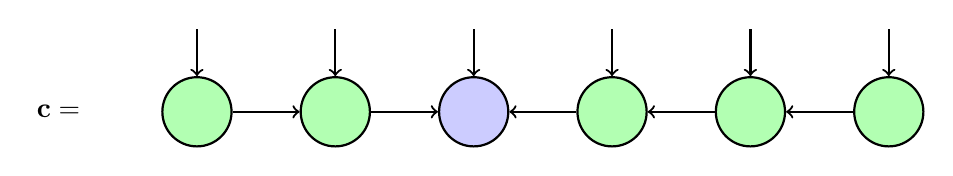
\begin{tikzpicture}[x=2em, y=2em, thick]
                \node (f) at (-2.5, 0) {\normalsize$\vb{c} = $};
                \node[basis] (h1) at (0,   0) {};
                \node[basis] (h2) at (2.5, 0) {};
                \node[state] (h3) at (5,   0) {};
                \node[basis] (h4) at (7.5, 0) {};
                \node[basis] (h5) at (10, 0) {};
                \node[basis] (h6) at (12.5, 0) {};
                \draw[->]  (h1)--(h2);
                \draw[->]  (h2)--(h3);
                \draw[<-]  (h3)--(h4);
                \draw[<-]  (h4)--(h5);
                \draw[<-]  (h5)--(h6);
                \draw[<-]  (h1) to (0,   1.5);
                \draw[<-]  (h2) to (2.5, 1.5);
                \draw[<-]  (h3) to (5,   1.5);
                \draw[<-]  (h4) to (7.5, 1.5);
                \draw[<-]  (h5) to (10, 1.5);
                \draw[<-]  (h6) to (12.5, 1.5); 
            \end{tikzpicture}
        \end{center}
        For a complete binary tree, the space for saving a wavefunction is $\order{dn^3}$ floats, if $n_{\ell} = \order{n}$ for all $\ell$.

        Generally, if $\rank{} \leqslant p$ for all nodes, the space for saving a wavefunction is of $\order{d n^p}$.
    \end{frame}

    \begin{frame}{Equations of Motion}
        \begin{center}
            \LARGE
            $\iu \hbar$
            \vcenteredhbox{
                \tiny
                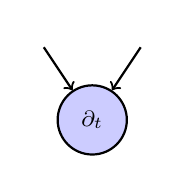
\begin{tikzpicture}[x=2em, y=2em, thick]
                    \node[state] (0)  at (0, 0) {\footnotesize$\partial_t$};
                    \node (11) at (-1, 1.5) {};
                    \node (12) at ( 1, 1.5) {};
                    \draw[->]  (11)--(0);
                    \draw[->]  (12)--(0);
                \end{tikzpicture}
            }
            $=$
            \vcenteredhbox{
                \tiny
                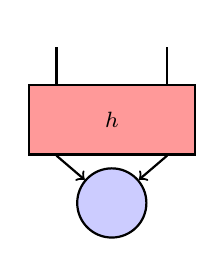
\begin{tikzpicture}[x=2em, y=2em, thick]
                    \node[operator, minimum width=6em] (0) at (0, 0) {\footnotesize$h$};
                    \node (11) at (-1, 1.5) {};
                    \node (12) at ( 1, 1.5) {};
                    \node[state] (a) at (0, -1.5) {};
                    \draw (11)--(11 |- 0.north) (12)--(12 |- 0.north);
                    \draw[<-]  (a)--(11 |- 0.south);
                    \draw[<-]  (a)--(12 |- 0.south);
                \end{tikzpicture}
            }
        \end{center}
        \begin{center}
            \LARGE
            $\iu \hbar$
            \vcenteredhbox{
                \tiny
                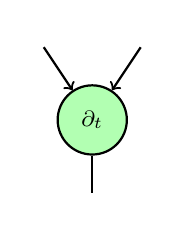
\begin{tikzpicture}[x=2em, y=2em, thick]
                    \node[basis] (0) at (0, 0) {\footnotesize$\partial_t$};
                    \node (11) at (-1, 1.5) {};
                    \node (12) at ( 1, 1.5) {};
                    \node (13) at (0, -1.5) {};
                    \draw[->]  (11)--(0);
                    \draw[->]  (12)--(0);
                    \draw (0)--(13);
                \end{tikzpicture}
            }
            $=$
            \vcenteredhbox{
                \tiny
                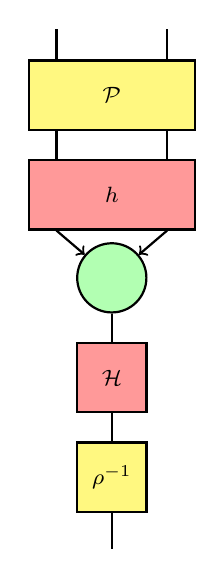
\begin{tikzpicture}[x=2em, y=2em, thick]
                    \node[operator, minimum width=6em] (0) at (0, 0) {\footnotesize$h$};
                    \node (11) at (-1, 1.5) {};
                    \node (12) at ( 1, 1.5) {};
                    \node[operator] (13) at (0, -3.3) {\footnotesize$\mathcal{H}$};
                    \node[other] (14) at (0, -5.1) {\footnotesize$\rho^{-1}$};
                    \node[other, minimum width=6em] (15) at (0, 1.8) {\footnotesize$\mathcal{P}$};
                    \node[basis] (a) at (0, -1.5) {};
                    \draw[<-]  (a)--(11 |- 0.south);
                    \draw[<-]  (a)--(12 |- 0.south);
                    \draw (a)--(13);
                    \draw (13)--(14);
                    \draw (11 |- 15.south)--(11 |- 0.north) (12 |- 15.south)--(12 |- 0.north);
                    \draw (11 |- 15.north)--(-1, 3) (12 |- 15.north)--(1, 3);
                    \draw (14)--(0, -6.4);
                \end{tikzpicture}
            }
        \end{center}
    \end{frame}

    \begin{frame}{Structure of $\vb{H}$}
        \begin{itemize}
            \item Matrix product operators (MPOs)
            \begin{center}
                \tiny
                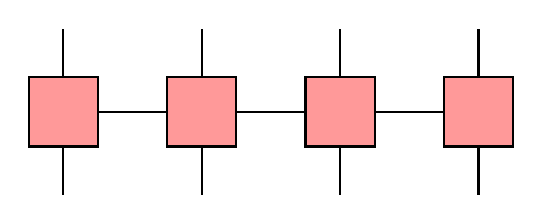
\begin{tikzpicture}[x=2em, y=2em, thick]
                    \node[operator] (h1) at (0,   0) {};
                    \node[operator] (h2) at (2.5, 0) {};
                    \node[operator] (h3) at (5,   0) {};
                    \node[operator] (h4) at (7.5, 0) {};
                    \draw (h1)--(h2) (h2)--(h3) (h3)--(h4);
                    \draw (h1) to (0,   1.5) (h1) to (0,   -1.5); 
                    \draw (h2) to (2.5, 1.5) (h2) to (2.5, -1.5);
                    \draw (h3) to (5,   1.5) (h3) to (5,   -1.5); 
                    \draw (h4) to (7.5, 1.5) (h4) to (7.5, -1.5); 
                \end{tikzpicture}
            \end{center}
            \item Summation of products of operators
            \begin{center}
                \tiny
                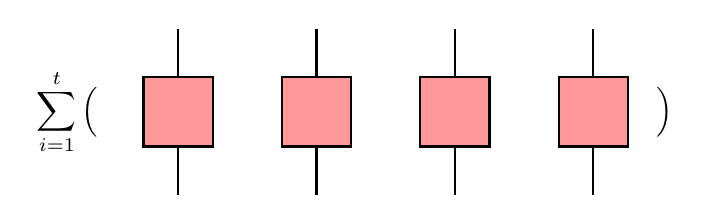
\begin{tikzpicture}[x=2em, y=2em, thick]
                    \node (f) at (-2, 0) {\normalsize$\displaystyle\sum_{i=1}^t\Big($};
                    \node (f) at (8.8, 0) {\normalsize$\Big)$};
                    \node[operator] (h1) at (0,   0) {};
                    \node[operator] (h2) at (2.5, 0) {};
                    \node[operator] (h3) at (5,   0) {};
                    \node[operator] (h4) at (7.5, 0) {};
                    \draw (h1) to (0,   1.5) (h1) to (0,   -1.5); 
                    \draw (h2) to (2.5, 1.5) (h2) to (2.5, -1.5);
                    \draw (h3) to (5,   1.5) (h3) to (5,   -1.5); 
                    \draw (h4) to (7.5, 1.5) (h4) to (7.5, -1.5); 
                \end{tikzpicture}
            \end{center}
        \end{itemize}
    \end{frame}

    \begin{frame}{Equations of Motion (Cont'd)}
        where for all nodes, w.\,l.\,o.\,g., choose one term in $\vb{H}$ and one node as an example:
        \begin{center}
            \LARGE
            \vcenteredhbox{\tiny
                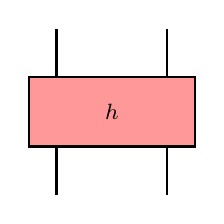
\begin{tikzpicture}[x=2em, y=2em, thick]
                    \node (11) at (-1, 1.5) {};
                    \node (12) at ( 1, 1.5) {};
                    \node[operator, minimum width=6em] (15) at (0, 1.5) {\footnotesize$h$};
                    \draw (11 |- 15.south)--(-1, 0) (12 |- 15.south)--(1, 0);
                    \draw (11 |- 15.north)--(-1, 3) (12 |- 15.north)--(1, 3);
                \end{tikzpicture}
            }
            \color{red!30!blue}{$\Leftarrow$}
            \color{black}
            \vcenteredhbox{\tiny
                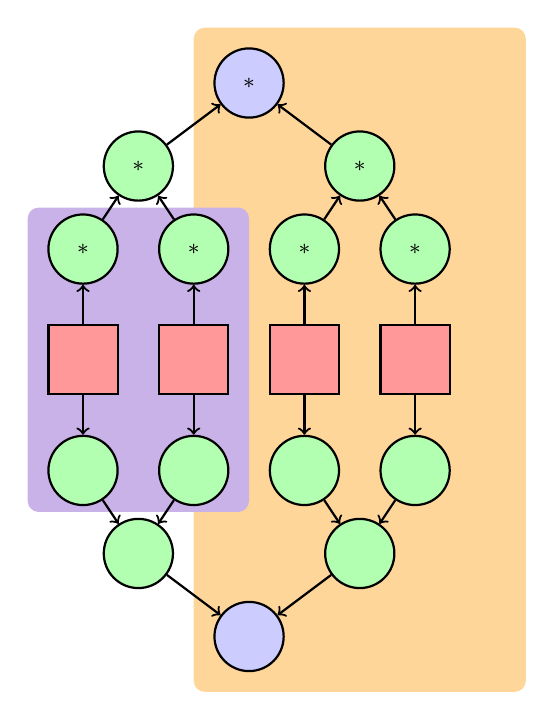
\begin{tikzpicture}[x=2em, y=2em, thick]
                    \node[
                        fill=red!40!yellow!40, minimum width=12em, minimum height=24em, rounded corners
                    ] (bg2) at (2,0) {};
                    \node[
                        fill=red!30!blue!30, minimum width=8em, minimum height=11em, rounded corners
                    ] (bg1) at (-2,0) {};
                    \node[state] (0)  at (0, -5) {};
                    \node[basis] (11) at (-2, -3.5) {};
                    \node[operator] (h1) at (-3, 0) {};
                    \node[operator] (h2) at (-1, 0) {};
                    \node[operator] (h3) at ( 1, 0) {};
                    \node[operator] (h4) at ( 3, 0) {};
                    \node[basis] (12) at ( 2, -3.5) {};
                    \node[basis] (21) at (-3, -2) {};
                    \node[basis] (22) at (-1, -2) {};
                    \node[basis] (23) at ( 1, -2) {};
                    \node[basis] (24) at ( 3, -2) {};
                    \draw[->]  (11)--(0);
                    \draw[->]  (12)--(0);
                    \draw[->]  (21)--(11);
                    \draw[->]  (22)--(11);
                    \draw[->]  (23)--(12);
                    \draw[->]  (24)--(12);
                    \draw[<-]  (21) to (h1);
                    \draw[<-]  (22) to (h2);
                    \draw[<-]  (23) to (h3);
                    \draw[<-]  (24) to (h4);
                    \node[state] (0t)  at (0, 5) {\footnotesize$*$};
                    \node[basis] (11t) at (-2, 3.5) {\footnotesize$*$};
                    \node[basis] (12t) at ( 2, 3.5) {\footnotesize$*$};
                    \node[basis] (21t) at (-3, 2) {\footnotesize$*$};
                    \node[basis] (22t) at (-1, 2) {\footnotesize$*$};
                    \node[basis] (23t) at ( 1, 2) {\footnotesize$*$};
                    \node[basis] (24t) at ( 3, 2) {\footnotesize$*$};
                    \draw[->]  (11t)--(0t);
                    \draw[->]  (12t)--(0t);
                    \draw[->]  (21t)--(11t);
                    \draw[->]  (22t)--(11t);
                    \draw[->]  (23t)--(12t);
                    \draw[->]  (24t)--(12t);
                    \draw[<-]  (21t) to (h1);
                    \draw[<-]  (22t) to (h2);
                    \draw[<-]  (23t) to (h3);
                    \draw[<-]  (24t) to (h4);
                \end{tikzpicture}
            }
            \color{red!40!yellow}{$\Rightarrow$}
            \color{black}
            \vcenteredhbox{\tiny
                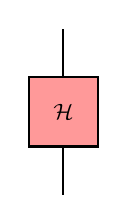
\begin{tikzpicture}[x=2em, y=2em, thick]
                    \node[operator] (14) at (0, 0) {\footnotesize$\mathcal{H}$};
                    \draw (14)--(0, 1.5) (14)--(0, -1.5);
                \end{tikzpicture}
            }
        \end{center}
    \end{frame}

    \begin{frame}{Equations of Motion (Cont'd)}
        and
        \begin{center}
            \LARGE
            \vcenteredhbox{
                \tiny
                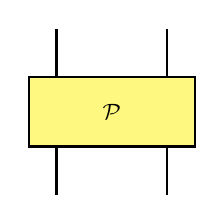
\begin{tikzpicture}[x=2em, y=2em, thick]
                    \node (11) at (-1, 1.5) {};
                    \node (12) at ( 1, 1.5) {};
                    \node[other, minimum width=6em] (15) at (0, 1.5) {\footnotesize$\mathcal{P}$};
                    \draw (11 |- 15.south)--(-1, 0) (12 |- 15.south)--(1, 0);
                    \draw (11 |- 15.north)--(-1, 3) (12 |- 15.north)--(1, 3);
                \end{tikzpicture}
            }
            $= 1-$
            \vcenteredhbox{
                \tiny
                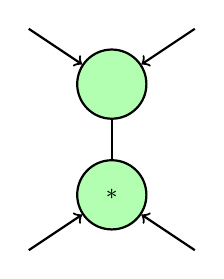
\begin{tikzpicture}[x=2em, y=2em, thick]
                    \node[basis] (at) at (0, 0) {\footnotesize$*$};
                    \node[basis] (a) at (0, 2) {};
                    \draw (a)--(at);
                    \draw[<-]  (a) --(-1.5, 3);
                    \draw[<-]  (a) --( 1.5, 3);
                    \draw[<-]  (at)--( 1.5, -1);
                    \draw[<-]  (at)--(-1.5, -1);
                \end{tikzpicture}
            }
            \vfill
            \vcenteredhbox{
                \tiny
                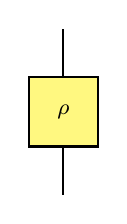
\begin{tikzpicture}[x=2em, y=2em, thick]
                    \node[other] (14) at (0, 0) {\footnotesize$\rho$};
                    \draw (14)--(0, 1.5) (14)--(0, -1.5);
                \end{tikzpicture}
            }
            $=$
            \vcenteredhbox{
                \tiny
                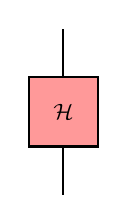
\begin{tikzpicture}[x=2em, y=2em, thick]
                    \node[operator] (14) at (0, 0) {\footnotesize$\mathcal{H}$};
                    \draw (14)--(0, 1.5) (14)--(0, -1.5);
                \end{tikzpicture}
            }
            $\eval{\huge}_{
                \vcenteredhbox{
                    \tiny
                    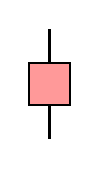
\begin{tikzpicture}[x=2em, y=2em, thick]
                        \node[operator, minimum width=1.5em, minimum height=1.5em] (14) at (0, 0) {};
                        \draw (14)--(0, 1) (14)--(0, -1);
                    \end{tikzpicture}
                }=1}
            $
        \end{center}
        Time complexity: if $\rank{} \leqslant p$ for all nodes, then a step of multiplication is of $\order{t p d n^{p+1}}$;

        Space complexity: $\order{t p d n^2 + d n^p}$.
    \end{frame}

    \begin{frame}{Example: 2-D harmonic oscillator}
        \footnotesize{
            $V = \frac{1}{2}x^2 + \frac{1}{2}y^2 + \frac{1}{4}xy$ (all in a.\,u.).
        
            Start from the ground state when $V = \frac{1}{2}x^2 + \frac{1}{2}y^2$. Use Sine-DVR as the (primitive) basis set and $n=40$, $L=10$.
        }
        \begin{figure}
            \includegraphics[width=0.6\textwidth]{autocorr_MCTDH.pdf}
            \caption{$|a(t)|$ -- $t$ (using RK45 as ODE solver, $\Delta t = 0.001~\text{a.\,u.}$)}
        \end{figure}
    \end{frame}

    \section{MCTDH vs. DMRG}

    \begin{frame}{Structure of Wavefunction: a TN perspective}
        \begin{itemize}
            \item MCTDH
            \begin{center}
                \tiny
                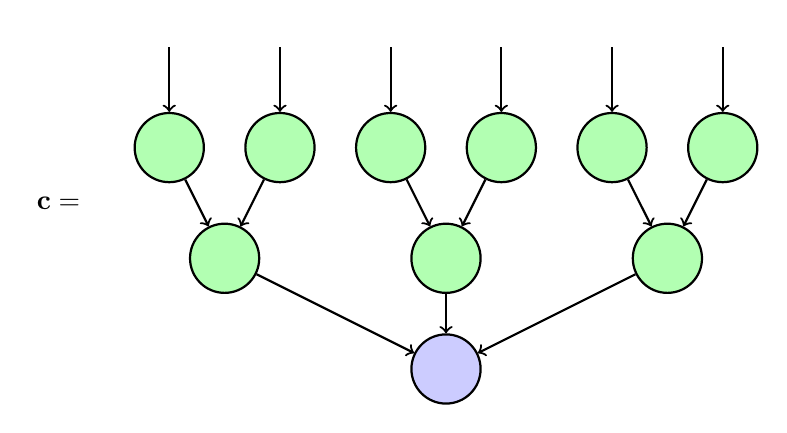
\begin{tikzpicture}[x=2em, y=2em, thick]
                    \node (f) at (-7, 2.5) {\normalsize$\vb{c} = $};
                    \node[state] (a) at (0, -0.5) {\pf};
                    \node[basis] (11) at (-4, 1.5) {\pf};
                    \node[basis] (12) at ( 0, 1.5) {\pf};
                    \node[basis] (13) at ( 4, 1.5) {\pf};
                    \node[basis] (21) at (-5, 3.5) {};
                    \node[basis] (22) at (-3, 3.5) {};
                    \node[basis] (23) at (-1, 3.5) {};
                    \node[basis] (24) at ( 1, 3.5) {};
                    \node[basis] (25) at ( 3, 3.5) {};
                    \node[basis] (26) at ( 5, 3.5) {};
                    \node (31) at (-5, 5.5) {};
                    \node (32) at (-3, 5.5) {};
                    \node (33) at (-1, 5.5) {};
                    \node (34) at ( 1, 5.5) {};
                    \node (35) at ( 3, 5.5) {};
                    \node (36) at ( 5, 5.5) {};
                    \draw[<-]  (a)--(11);
                    \draw[<-]  (a)--(12);
                    \draw[<-]  (a)--(13);
                    \draw[<-]  (11) to (21);
                    \draw[<-]  (11) to (22);
                    \draw[<-]  (12) to (23);
                    \draw[<-]  (12) to (24);
                    \draw[<-]  (13) to (25);
                    \draw[<-]  (13) to (26);
                    \draw[<-]  (21) to (31);
                    \draw[<-]  (22) to (32);
                    \draw[<-]  (23) to (33);
                    \draw[<-]  (24) to (34);
                    \draw[<-]  (25) to (35);
                    \draw[<-]  (26) to (36);
                \end{tikzpicture}
            \end{center}
            \item DMRG
            \begin{center}
                \tiny
                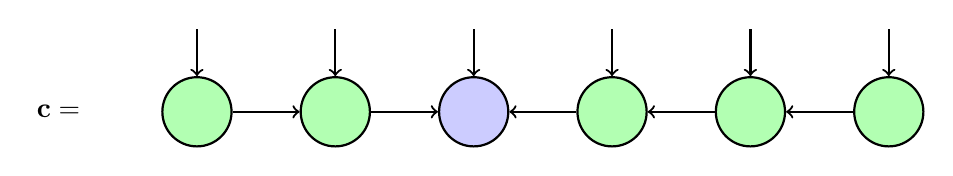
\begin{tikzpicture}[x=2em, y=2em, thick]
                    \node (f) at (-2.5, 0) {\normalsize$\vb{c} = $};
                    \node[basis] (h1) at (0,   0) {};
                    \node[basis] (h2) at (2.5, 0) {};
                    \node[state] (h3) at (5,   0) {};
                    \node[basis] (h4) at (7.5, 0) {};
                    \node[basis] (h5) at (10, 0) {};
                    \node[basis] (h6) at (12.5, 0) {};
                    \draw[->]  (h1)--(h2);
                    \draw[->]  (h2)--(h3);
                    \draw[<-]  (h3)--(h4);
                    \draw[<-]  (h4)--(h5);
                    \draw[<-]  (h5)--(h6);
                    \draw[<-]  (h1) to (0,   1.5);
                    \draw[<-]  (h2) to (2.5, 1.5);
                    \draw[<-]  (h3) to (5,   1.5);
                    \draw[<-]  (h4) to (7.5, 1.5);
                    \draw[<-]  (h5) to (10, 1.5);
                    \draw[<-]  (h6) to (12.5, 1.5); 
                \end{tikzpicture}
            \end{center}
        \end{itemize}
    \end{frame}

    \begin{frame}{Algorithm: Differnet Choices}
        \begin{center}
            \begin{tabular}{r|ll}
                      & TDSE                 & TISE \\\hline
                DMRG  & Based on propergators & DMRG1, DMRG2 \\
                MCTDH & Based on DFVP        & Self-consistent \\
            \end{tabular}            
        \end{center}

        \begin{itemize}
            \item[$\circ$] Other combinations?
        \end{itemize}
    \end{frame}

    \begin{frame}{Conclusions}
        \begin{itemize}
            \item The structure of wavefunctions in  MCTDH and DMRG can be unified in tensor network theory;
            \item The algorithms used in traditional MCTDH and DMRG are interchangeable in principle;
            \item The proper structure of wavefunctions in a specific problem needs further studying.
        \end{itemize}
    \end{frame}

    \begin{frame}{Acknowledgments}
        \begin{center}
            \large
            Thank you for your listening!
        \end{center}
    \end{frame}

    
    \begin{frame}{Normalization}
        General normalization condition at the $\ell$-th node:
        \begin{center}
            \tiny
            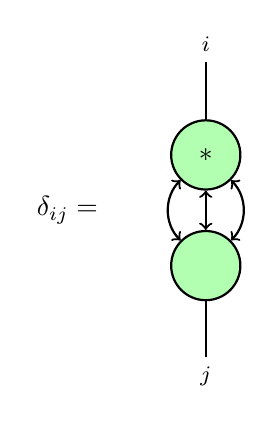
\begin{tikzpicture}[x=2em, y=2em, thick]
                \node[basis] (a) at (0, 0) {};
                \node (f) at (-2.5, 1) {\normalsize$\delta_{ij} =$};
                \node[basis] (at) at (0, 2) {\normalsize$*$};
                \node (i) at (0, 4) {\footnotesize$i$};
                \node (j) at (0, -2) {\footnotesize$j$};
                \draw[<->]  (a)--(at);
                \draw[<->]  (a) to[out=45, in=-45]   (at);
                \draw[<->]  (a) to[out=135, in=-135] (at);
                \draw (at)--(i) (a)--(j);
            \end{tikzpicture}
            \hspace{0.1\textwidth}
            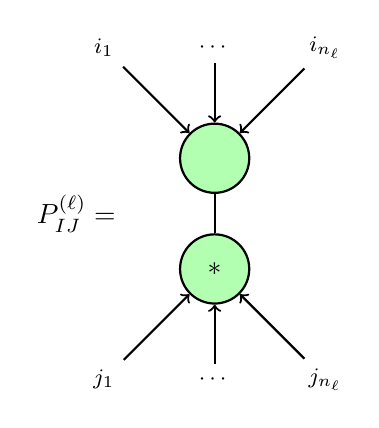
\begin{tikzpicture}[x=2em, y=2em, thick]
                \node (f) at (-2.5, 1) {\normalsize$P^{(\ell)}_{IJ} =$};
                \node[basis] (a) at (0, 0) {\normalsize$*$};
                \node[basis] (at) at (0, 2) {};
                \node (i1) at (-2, 4) {\footnotesize$i_1$};
                \node (i2) at ( 0, 4) {\footnotesize$\cdots$};
                \node (i3) at ( 2, 4) {\footnotesize$i_{n_\ell}$};
                \node (j1) at (-2, -2) {\footnotesize$j_1$};
                \node (j2) at ( 0, -2) {\footnotesize$\cdots$};
                \node (j3) at ( 2, -2) {\footnotesize$j_{n_\ell}$};
                \draw (a)--(at);
                \draw[<-]  (a)--(j1);
                \draw[<-]  (a)--(j2);
                \draw[<-]  (a)--(j3);
                \draw[<-]  (at)--(i1);
                \draw[<-]  (at)--(i2);
                \draw[<-]  (at)--(i3);
            \end{tikzpicture}
        \end{center}
    \end{frame}

    \begin{frame}{Normalization (Cont'd)}
        In order to hold all general normalization conditions during the propergation, one must have
        \begin{center}
            \tiny
            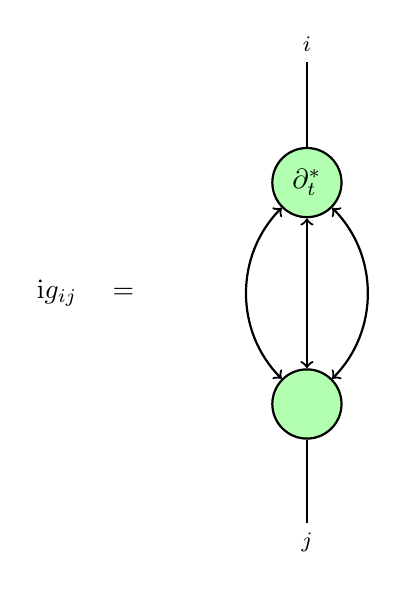
\begin{tikzpicture}[x=2em, y=2em, thick]
                \node[basis] (a) at (0, -1) {\phantom{\normalsize$\partial_t^*$}};
                \node (f) at (-4, 1) {\normalsize$\iu g_{ij} \quad =$};
                \node[basis] (at) at (0, 3) {\normalsize$\partial_t^*$};
                \node (i) at (0, 5.5) {\footnotesize$i$};
                \node (j) at (0, -3.5) {\footnotesize$j$};
                \draw[<->]  (a)--(at);
                \draw[<->]  (a) to[out=45, in=-45]   (at);
                \draw[<->]  (a) to[out=135, in=-135] (at);
                \draw (at)--(i) (a)--(j);
            \end{tikzpicture}
        \end{center}
        where $\vb{g}$ is Hermitian. For simplicity, choose $\vb{g} = 0$.
    \end{frame}

\end{document}
